%%%%%%%%%%%%%%%%%%%%%%%%%%%%%%%%%%%%%%%%%%%%%%%%%%%%%%%%%%%%%%%%%%%%%%%%%%%%%%%%
%Objetivo: Descrever a implementação de uma extensão para uma FGRM de modo a
%avaliar o impacto este tipo de melhoria pode causar neste tipo de ferramenta.
%Autores: Vagner Clementino <vagnercs@dcc.ufmg.br>
%		  Rodolfo Resende <rodolfo@dcc.ufmg.br>
%Criação: dom fev 26 12:49:27 BRT 2017
%Modificação: dom mai 14 18:17:37 -03 2017
%Revisão: dom mar 12 09:35:34 BRT 2017
%%%%%%%%%%%%%%%%%%%%%%%%%%%%%%%%%%%%%%%%%%%%%%%%%%%%%%%%%%%%%%%%%%%%%%%%%%%%%%%%
\chapter{Implementação de uma Extensão para FGRM}
\label{ch:implemtacao_extensao}

\section{Introdução}
\label{sec:implemtacao_extensao_intro}

% Durante esta dissertação discutimos que as funcionalidades oferecidas FGRMs
% atendem as expectativas dos seus usuários. Todavia, após resultados como aqueles
% obtidos nos Capítulo~\ref{ch:pesquisa-profissionais} e~\ref{ch:sug_melhoria},
% verificamos que exite um espaço para melhorias das funcionalidades existentes ou
% mesmo para a proposição de novas. Alguns estudos vêm seguindo esta tendência,
% especialmente explorando a capacidade de extensão propiciada por algumas FGRMs.
% A extensão \textit{Buglocalizer}~\cite{Thung:2014:BIT:2635868.2661678}, criada
% para a ferramenta Bugzilla, possibilita a localização dos arquivos do código
% fonte que estão relacionados ao defeito relatado. A ferramenta extrai texto dos
% campos de sumário e descrição da RM\@. Este texto é comparado com o código fonte
% por meio de técnicas de Recuperação da Informação.

% Na mesma linha, o \textit{NextBug}~\cite{101186} é uma extensão para o Bugzilla
% que recomenda novas RMs para o desenvolvedor com base na que ele esteja tratando
% atualmente. Na ferramenta proposta por Thung e
% outros~\cite{Thung:2014:DIT:2642937.2648627} o foco é na determinação de
% defeitos duplicados. A contribuição deste trabalho é a integração do estado da
% arte de técnicas não supervisionadas para detecção de RMs duplicadas.

% Esta dissertação se propôs a contribuir com a melhoria das funcionalidades das
% FGRMs mediante a apresentação e discussão de um conjunto de recomendações no
% Capitulo~\ref{ch:sug_melhoria}. Apesar de ter sido conduzido um processo de
% avaliação das recomendações, cujo resultado demonstrou uma boa aceitação dos
% participantes, optamos por analisar o impacto da implementação de uma das
% sugestões propostas.

% Idealmente gostaríamos de transformar todas as sugestões em extensões de
% funcionalidades para as FGRMs. Não há razões que justifiquem a priorização de
% implementação de uma recomendação sobre outra. Entretanto, após alguns ensaios e
% combinando de maneira mais intuitiva do que seguindo um fluxo de critérios,  foi
% investido mais esforço no desenvolvimento de uma extensão para o suporte à
% qualidade de relato. A extensão proposta tem por objetivo ser uma Prova de
% Conceito, ou seja, demostrar com o fim de verificar que o conceito proposto
% possui certo \textit{potencial} prático. Na próxima seção apresentamos uma breve
% discussão sobre o problema da baixa qualidade do relato no contexto das FGRMs.

Neste capítulo complementamos a contribuição do Capítulo 5 com a discussão de
aspectos de implementação. Este capítulo apresenta a implementação da Sugestão
\#1 na plataforma Github. A escolha da Sugestão \#1 e da plataforma Github
envolve mais aspectos de serem convenientes do que algum tipo de decisão formal.

\section{Qualidade do Relato de uma RM}
\label{sec:avaliando_a_qualidade_do_relato_de_uma_rm}

É possível considerar que as informações mais relevantes estejam no relato de
uma RM, que é o atributo que representa o texto redigido pelo Reportador.
Sabemos que o ato de reportar uma RM pode ser realizado por um usuário do
software ou por um membro da equipe de desenvolvimento ou manutenção. Por esta
razão, podemos encontrar Reportadores com diferentes níveis de conhecimento
sobre o sistema. Esta situação pode provocar um efeito colateral: a baixa
qualidade do texto no relato de uma RM, como por exemplo a falta da informação
necessária para sua solução.

Alguns estudos afirmam que a baixa qualidade do relato prejudicam o andamento do
projeto mais do que RMs duplicadas~\cite{bettenburg2007quality}. No estudo
realizado por Bettenburg e outros~\cite{bettenburg2008makes} foi desenvolvido um
levantamento com questionário entre desenvolvedores e usuários de três projetos
de código aberto\footnote{Apache (\url{http://www.apache.org/}), Eclipse
    (\url{https://www.eclipse.org}) e Mozilla (\url{https://www.mozilla.org})}.
O objetivo era coletar informação de modo a verificar o que produziria um bom
relato. Os resultados demonstraram que, do ponto de vista dos desenvolvedores,
são consideradas informações úteis para estar no relato de uma RM\@:

\begin{itemize}
    \item a sequência de ações executadas até o aparecimento da falha, também
        conhecida como \textit{etapas para reproduzir};
    \item a cadeia de registros de ativação (stack traces) que corresponde à
        descrição das chamadas de funções ou métodos que ocorreram antes do
        aparecimento da falha.
\end{itemize}

No estudo proposto por Zimmermann e outros~\cite{5070993} é discutida a
importância de que a informação descrita em uma RM seja relevante e completa a
fim de que o problema relatado seja resolvido rapidamente.  Contudo, na prática,
a informação apenas chega ao desenvolvedor com a qualidade requerida após
diversas interações com o usuário afetado. Com o objetivo de minimizar este
problema os autores propõem um conjunto de diretrizes para a construção de uma
extensão capaz de reunir informações relevantes a partir do usuário além de
identificar arquivos que precisam ser corrigidos para resolver o defeito.

Conforme exposto, a utilização de uma extensão que suporte a melhoria da
qualidade do relato pode resultar nas seguintes vantagens: redução no tempo
necessário para análise do que foi solicitado na RM\@; facilidade na
identificação de RMs duplicadas; melhor disciplina dos Reportadores sobre a boa
prática de fornecer um relato com maior qualidade. Estas vantagens têm impacto
no custo e qualidade do software produzido.

\section{Uma Extensão para Suporte à Qualidade do Relato}
\label{sec:uma_extensao_suporte_qualidade_relato}

Considerando as vantagens de analisar a qualidade do relato de uma RM,
desenvolvemos uma extensão para o módulo de gerenciamento de RMs da plataforma
Github\footnote{\url{https://guides.github.com/features/issues/}}. De uma
maneira geral, a extensão proposta realiza a análise do relato contido em uma RM
e com base nele gera uma realimentação contendo ``dicas'' que podem melhorar a
qualidade da informação prestada. Nas próximas seções apresentamos com mais
detalhe o desenho e funcionamento da extensão proposta.

% \begin{description}
% 	\item[Questão 01:] Qual impacto da inclusão de uma extensão para o suporte à
% 		qualidade do relato pode ter no tempo necessário para análise de uma
% 		RM\@?
% 	\item[Questão 02:] Existe relação entre a frequência que um participante
% 		cria uma RM e a qualidade do relato?
% 	\item[Questão 03:] Do ponto de vista dos profissionais envolvidos em
% 		manutenção de software qual o impacto da inclusão de uma extensão para o
% 		suporte à qualidade do relato no processo de manutenção de software?
% \end{description}

% Na \textit{Questão 01} estamos interessados em verificar se a inclusão de uma
% extensão deste tipo pode atrasar o processo de resolução de uma RM por conta da
% eventual sobrecarga que a análise da qualidade do relato pode causar. A
%  \textit{Questão 02} possui o foco em avaliar se aquelas pessoas que criam RM com
% maior frequência em determinado projeto possuem uma qualidade do relato superior
% daqueles que fazem isso eventualmente. Por fim, na \textit{Questão 03} queremos
% entender os prós e contras que a implantação deste tipo de extensão pode
% produzir no processo de manutenção de software tomando como base a opinião de
% profissionais da área.

\subsection{Desenho da Extensão}
\label{sub:desenho_da_extensao}

O objetivo da extensão é analisar de maneira automatizada a qualidade do relato
de uma \textit{RM} em repositórios do GitHub. No contexto da extensão proposta,
o elemento correspondente ao conceito de uma RM nesta dissertação representa o
elemento \textit{issue} no âmbito da plataforma Github. Um Repositório é o
elemento mais básico do GitHub e contém os arquivos do projeto (incluindo
documentação) e armazena o histórico de revisões de cada
arquivo\footnote{\url{https://help.github.com/articles/github-glossary/}}. A
execução da extensão resulta em um conjunto de dicas para o responsável por
redigir a \textit{RM} com o intuito de melhorar a qualidade da informação
fornecida no relato, por esta razão recebeu o nome de \textit{IssueQuality}.

\subsubsection{Visão Geral}
\label{ssub:implementacao_extensao_visao_geral}

A extensão proposta pode ser vista como um cliente para API do
Github\footnote{\url{https://api.github.com/}} que possibilita analisar a
qualidade da informação fornecida no relato. Uma visão geral sobre o
funcionamento da \textit{IssueQuality} pode ser visualizada na
Figura~\ref{fig:diagrama_funcionamento_issuequality}. A partir de uma lista
pré-definida de repositórios (1) a extensão solicita, através da API do Github
(2), o conjunto de \textit{RMs} que estão com a situação \textit{``aberta''}
(etapas 3 e 4). Para cada uma das \textit{RMs} recebidas, a ferramenta cria
um comentário por meio da API (5) que é registrado e armazenado no repositório
de RMs do Github (etapas 6 e 7). A partir do comentário gerado o próprio Github
se encarrega de notificar (8) o responsável por relatar a \textit{RM} (9). A
partir desta notificação espera-se que o responsável inclua a informação
solicitada mediante a criação de um novo comentário.

\begin{figure}[htpb]
    \centering
    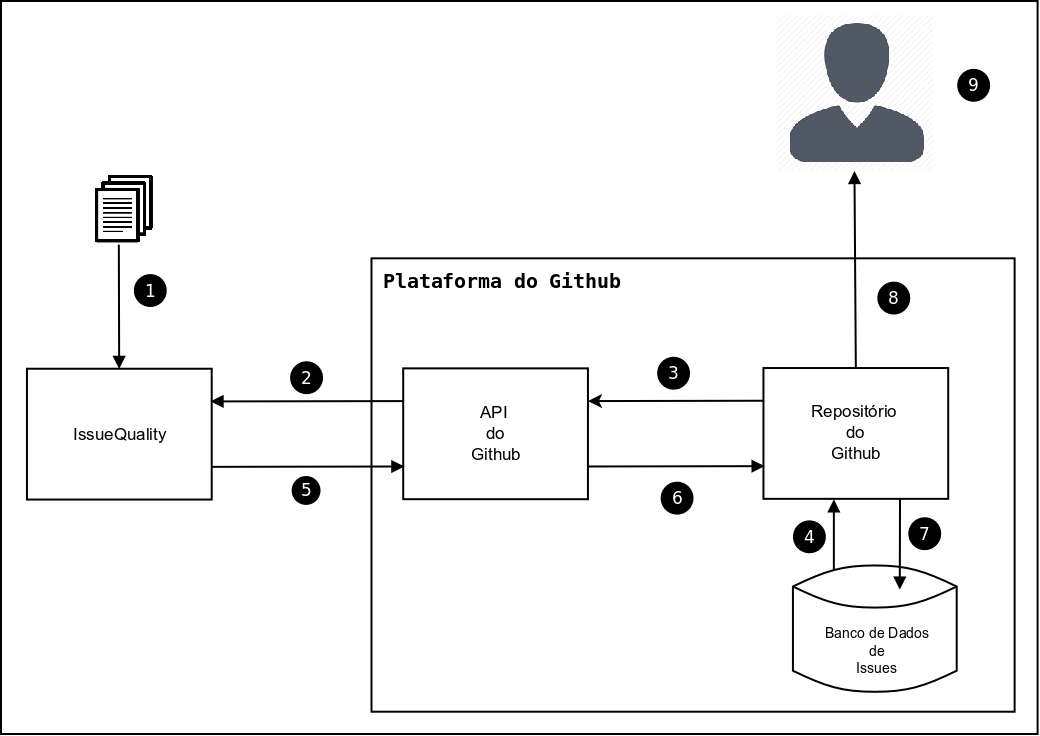
\includegraphics[width=0.7\linewidth]{chapter-implementacao-extensoes-fgrm/img/diagrama_funcionamento_issuequality.png}
    \caption{Visão geral do funcionamento da extensão \textit{IssueQuality}}
\label{fig:diagrama_funcionamento_issuequality}
\end{figure}

Para gerar o comentário descrito anteriormente, a extensão avalia alguns
atributos do texto que compõe o relato da RM\@. Os detalhes de como estes
atributos são analisados e o comentário construído estão descritos na próxima
seção.

\subsubsection{Análise da Qualidade do Relato}
\label{ssub:implementacao_extensao_analise_qualidade_do_relato}

Para cada RM analisada a extensão cria um \textit{vetor de características} que
armazena uma pontuação para cada atributo do texto que será analisado. A análise
dos atributos utilizam da sintaxe da linguagem de marcação
Markdown\footnote{\url{https://help.github.com/categories/writing-on-github/}},
que é o padrão para as RMs dos repositórios no GitHub.

Conforme descrito, o resultado da análise feita pela extensão é uma
realimentação na forma de um comentário associado à RM\@. Em geral, ele é
composto de três partes: \textit{cabeçalho, corpo e dicas}. O cabeçalho
apresenta um texto padrão que é personalizado com o nome do usuário (login) no
Github do reportador. Ao utilizarmos a sintaxe \textit{\@[Github login]} o
próprio Github se encarrega de enviar um e-mail notificando o usuário sobre o
comentário. A Figura~\ref{fig:issue_original} exibe o cabeçalho padrão incluídos
nos comentários.

\begin{figure}[htpb]
    \centering
    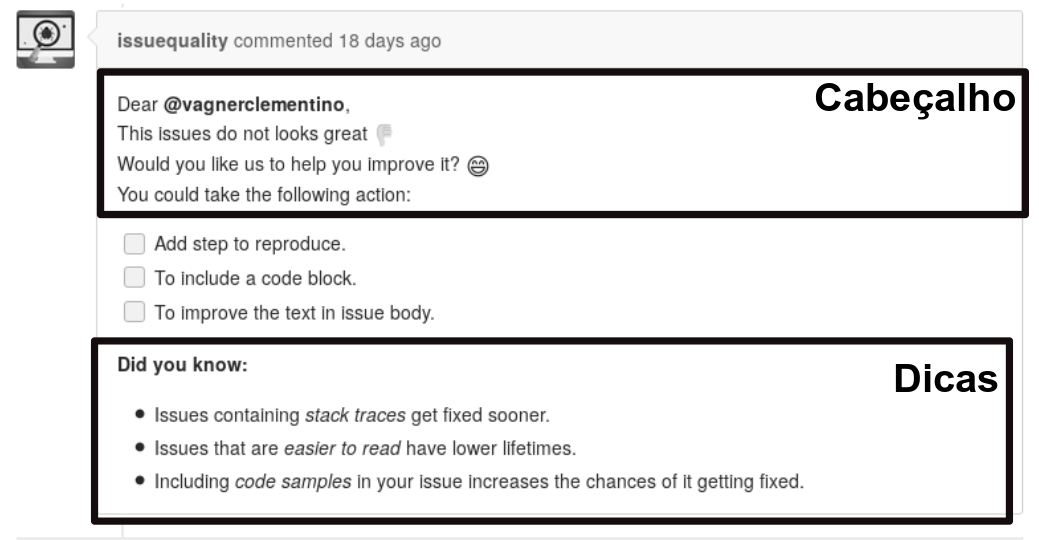
\includegraphics[width=0.8\linewidth]{chapter-implementacao-extensoes-fgrm/img/issue_original.png}
    \caption{Comentário produzido pela extensão IssueQuality com os cabeçalhos e
        dicas padrões.}
\label{fig:issue_original}
\end{figure}

Ao final do comentário é incluído um conjunto de dicas com objetivo de reforçar
os benefícios que a melhoria da qualidade do relato pode ter na solução da RM
correspondente, como por exemplo dizendo: \textit{``as RMs que são mais fáceis
    de serem lidas possuem um tempo de solução menor''}. Estas dicas foram
obtidas com base na literatura sobre melhoria da qualidade do relato,
especialmente nos trabalhos de Bettenburg e outros~\cite{bettenburg2007quality,
    bettenburg2008makes}. Na Figura~\ref{fig:issue_original} é possível
visualizar como algumas dicas são apresentadas.

O corpo é a parte dinâmica do comentário. Ele é construído incluindo fragmentos
de texto quando certos critérios de aceitação não foram atendidos.  Por exemplo,
caso não seja detectada a presença de \textit{``etapas para reproduzir''} no
relato de uma \textit{RM} o seguinte fragmento de texto é incluído no corpo
do comentário: \textit{``Add step to reproduce''}. Os atributos avaliados e os
critérios de aceitação estão descritos na
Tabela~\ref{tab:criterios_analise_qualidade_relato}.

\begin{table}[htpb]
\centering
\resizebox{\textwidth}{!}{%
\begin{tabular}{@{}cl@{}}
\toprule
\textbf{Atributo}             & \multicolumn{1}{c}{\textbf{Critério de Aceitação}}\\
\midrule
Completude de Palavras-chaves & Existência de uma lista representando as etapa
executadas até ocorrência do erro.         \\
Arquivos Anexados             & Pelo menos um arquivo anexado a RM
\\
Fragmentos de Código          & Existência de pelo menos um fragmento de código
no relato da RM\@.                       \\
Completude do Texto           & As palavras que compõe o relato da RM devem
fazer parte de pelo menos duas categorias. \\
Legibilidade do Texto         & Dois testes de legibilidade apresentarem valores
acima dos limiares.                      \\ \bottomrule
\end{tabular}%
}
\caption{Critérios de aceitação e forma de análise utilizados na análise de
    qualidade do relato.}
\label{tab:criterios_analise_qualidade_relato}
\end{table}

O corpo do comentário é produzido com análise dos seguintes atributos do relato
da RM\@: \textit{Etapas para Reproduzir, Arquivos Anexados, Fragmentos de
    Código, Completude do Texto e Legibilidade do Texto}. Estes atributos foram
baseados no estudo realizado por Bettenburg e outros~\cite{bettenburg2008makes}.
A seguir apresentamos os detalhes de como cada atributo é avaliado.

\paragraph{Etapas para Reproduzir:}
\label{par:etapas_para_reproduzir_}

Verifica se o reportador incluiu uma lista, na forma de itens, descrevendo as
etapas executadas até a ocorrência da falha. Para detectar este padrão a
extensão aproveita da linguagem Markdown, que é o padrão utilizado para redigir
o relato da \textit{RM}, e que possui uma sintaxe pré-definida para listas. O
padrão é detectado através da utilização de expressões regulares. Pode ocorrer
que o Reportador utilize outro formato para relatar as etapas executadas até a
ocorrência da falha, contudo, o fato da extensão exigir a informação através de
uma lista, pode criar no Reportador uma boa prática. Cabe ressaltar que uma
lista com etapas para reproduzir uma falha foi considerada uma das informações
mais relevantes de um relato~\cite{bettenburg2008makes}.

\paragraph{Arquivos Anexados:}
\label{par:arquivos_anexados}

Nesta dimensão avaliamos a existência de arquivos anexados à \textit{RM}, tais
como capturas de telas (screenshots) e cadeia de registros de ativação de
funções (stack trace). A detecção é realizada utilizando expressões regulares
que é a sintaxe padrão para o relato da
RM\footnote{\url{https://guides.github.com/features/mastering-markdown/}}. Não
houve avaliação sobre o conteúdo do anexo, contudo, conforme descrito na
Tabela~\ref{tab:criterios_analise_qualidade_relato}, uma mensagem é incluída no
corpo do comentário no caso de nenhum anexo ser detectado. A existência de
anexos em uma RM consta como uma das informações mais relevantes do ponto de
vistas dos desenvolvedores~\cite{bettenburg2008makes}.

\paragraph{Fragmentos de Código}
\label{par:fragmentos_de_código}

Este atributo de avaliação verifica se fragmentos de código foram adicionados no
relato da \textit{RM}. O processo de detecção faz uso de expressão regulares
e da sintaxe oferecida pela versão do Markdown utilizado pelo
Github\footnote{\url{https://guides.github.com/features/mastering-markdown/\#GitHub-flavored-markdown}}.
De forma similar aos atributos descritos anteriormente, a verificação de
fragmentos de código fonte é binária, ou seja, foi avaliada a existência ou não
de trecho de código.

\paragraph{Completude do Texto:}
\label{par:completude_de_palavras_chaves}

Nesta dimensão da avaliação há uma premissa que possa existir um vocabulário
comum no relato de diferentes RMs. Sendo assim, algumas palavras aparecem com
determinada frequência no relato de uma RM, independente do projeto. Com o
objetivo de compreender como as pessoas descrevem problemas de software, Ko e
outros~\cite{ko2006linguistic} analisaram o título de 200.000 RMs de cinco
projetos de código aberto desenvolvidos na linguagem Java. Nós empregamos esta
base de dados\footnote{Disponível para download em
    \url{http://www.cs.cmu.edu/~marmalade/reports.html.}} para construir uma
distribuição da frequência de ocorrências de palavras no relato de uma RM\@.  Em
uma primeira etapa, removemos as palavras de parada (stopwords), reduzimos as
vocábulos\footnote{Do inglês \textit{stemming} é o processo de reduzir palavras
    flexionadas (ou às vezes derivadas) ao seu tronco (stem), base ou raiz,
    geralmente uma forma da palavra escrita. Por exemplo um algoritmo de
    stemming reduz as palavras ``fishing'', ``fished'' e ``fisher'' para a raiz
    ``fish''.} e selecionamos as \textit{100} palavras com maior frequência. Em
seguida, categorizamos as palavras nos seguintes grupos:

\begin{itemize}

    \item itens de ação (do, work,open)
    \item relacionado com compilação (build, task)
    \item relacionado com documentação (support, help, content)
    \item comportamento esperado ou observável (fail, error, crash)
    \item relacionado com projeto (management, list)
    \item relacionado com código fontesource code-related (java, code, method)
    \item elementos da interface do usuário (menu, display, button)

\end{itemize}

\paragraph{Legibilidade do Texto}
\label{par:legibilidade_do_texto}

Por fim a extensão avalia o nível de legibilidade do texto com base em testes
largamente utilizados na literatura~\cite{Si:2001:SMS:502585.502695}. Os testes
são formulados para avaliar a legibilidade do texto, geralmente contando
sílabas, palavras e frases. Neste estudo utilizamos os testes de legibilidade
\textit{Flesch–Kincaid, Automated Readability Index \@-\@ ARI e Dale–Chall
    Readability Formula}. As avaliações foram selecionadas por apresentarem
metodologias distintas para determinar a legibilidade do texto.

O Flesch-Kincaid (FK) é baseado no número de sílabas das palavras que compõem as
sentenças do texto. Existem dois testes, o Flesch Reading Ease e Flesch–Kincaid
Grade Level, que diferem pelo fator de ponderação utilizado. A extensão utilizou
o Flesch Reading Ease que recebe um texto em língua inglesa e retorna um valor
inteiro representando a dificuldade de entendimento. Pontuações mais altas
indicam que o material é mais fácil de ler~\cite{kincaid1975derivation}. Desta
forma, foi considerada como legibilidade baixa uma pontuação \textit{menor do
    50}. Este valor foi baseado em uma tabela pré-definida pelo próprio
teste~\cite{kincaid1975derivation}.

O ARI considera o número de caracteres de cada palavra. O resultado do teste é
uma representação aproximada do grau de escolaridade no estilo K-12 dos Estados
Unidos necessário para compreender o texto~\cite{senter1967automated}. De
maneira aproximada, o grau 1 corresponde a idades 6\@-\@8. O nível de leitura 8
corresponde a jovem de 14 anos. O grau 12, o mais alto no ensino secundário dos
EUA, corresponde ao nível de leitura de 17 anos de idade.

Por outro lado, o teste Dale-Chall é baseado em um conjunto mínimo de palavras.
A fórmula usa uma lista de 3000 vocábulos que grupos de estudantes americanos de
quarta série poderiam entender de forma confiável, partindo-se da premissa que
qualquer palavra nessa lista não seja de difícil
compreensão~\cite{dale1948formula}. No caso dos testes ARI e Dale-Chall a
legibilidade será considerada ruim se o valor do teste \textit{for maior ou
    igual a 13}, ou seja, uma pessoa deveria estudar no mínimo 13 anos para
``entender''. Esta limiar foi utilizado no trabalho de Bettenburg e
outros~\cite{bettenburg2008makes}.

\section{Uso da Extensão em Projetos Reais}
\label{sec:avaliando_a_extensao_proposta}

A extensão descrita neste Capitulo foi desenvolvida como prova de conceito.
Neste sentido, o desenho e o desenvolvimento tiveram mais foco na viabilidade do
que estava sendo proposto do que melhorar ou sobrepor determinada solução do
estado da arte. Entretanto, com o objetivo de avaliar a extensão em um contexto
mais próximo do cotidiano de desenvolvedores, ela foi executada utilizando os
dados de \textit{RMs} de projetos código aberto hospedados no Github.

\subsection{Seleção dos Projetos}
\label{sub:implementacao_selecao_projetos}

Para realizarmos a execução da extensão usamos, por motivos já explicados, uma
amostra de conveniência composta de projetos hospedados na plataforma Github.
Para isso utilizamos os mesmos critérios descritos na
Seção~\ref{ssub:sug_melhoria_selecao_participantes}. As exceções foi que
incluímos a restrição de que o projeto fosse desenvolvido em Java e avaliamos os
dez primeiros projetos ordenados pelo critério ``most stars''. O condicionante
da linguagem Java é por conta de algumas decisões tomadas durante o
desenvolvimento da extensão que exigem a utilização da linguagem. Após aplicação
dos critérios descritos obtivemos os projetos apresentados na
Tabela~\ref{tab:projetos_utilizados}.

\begin{table}[htpb]
\centering
\resizebox{.7\textwidth}{!}{%
\begin{tabular}{@{}llcc@{}}
\toprule
\multicolumn{1}{c}{\textbf{Projeto}} & \textbf{Revisões} & \textbf{Ramificações} & \textbf{Lançamentos} \\ \midrule
elasticsearch & 27.118 & 94 & 174 \\
guava & 4.081 & 84 & 175 \\
spring-framework & 14575 & 12 & 106 \\ \bottomrule
\end{tabular}%
}
\caption{Projetos utilizados no testes de execução da extensão. Os dados
    apresentados têm como referência 23/04/2017.}
\label{tab:projetos_utilizados}
\end{table}

\subsubsection{O Processo de Execução}
\label{sub:implementacao_processo_execucao}

Para avaliarmos a extensão começamos por criar uma ramificação (fork) dos
projetos escolhidos. Este processo é realizado de forma automatizada pelo
Github, contudo, não realiza a cópia das \textit{RMs}, que no caso deste teste é
a informação mais relevante. Para transpor os dados das RMs foi desenvolvido um
processo automatizado que copiava o título e o relato (corpo da RM) do projeto
original para a sua ramificação. Para cada projeto realizamos a cópia de 100
\textit{RMs}. A Figura~\ref{fig:copia-de-issues} exibe uma \textit{RM} do
projeto Guava no lado esquerdo e sua cópia na ramificação criada. Como pode ser
observado título e o relato são idênticos.

\begin{figure}[htpb]
    \centering
    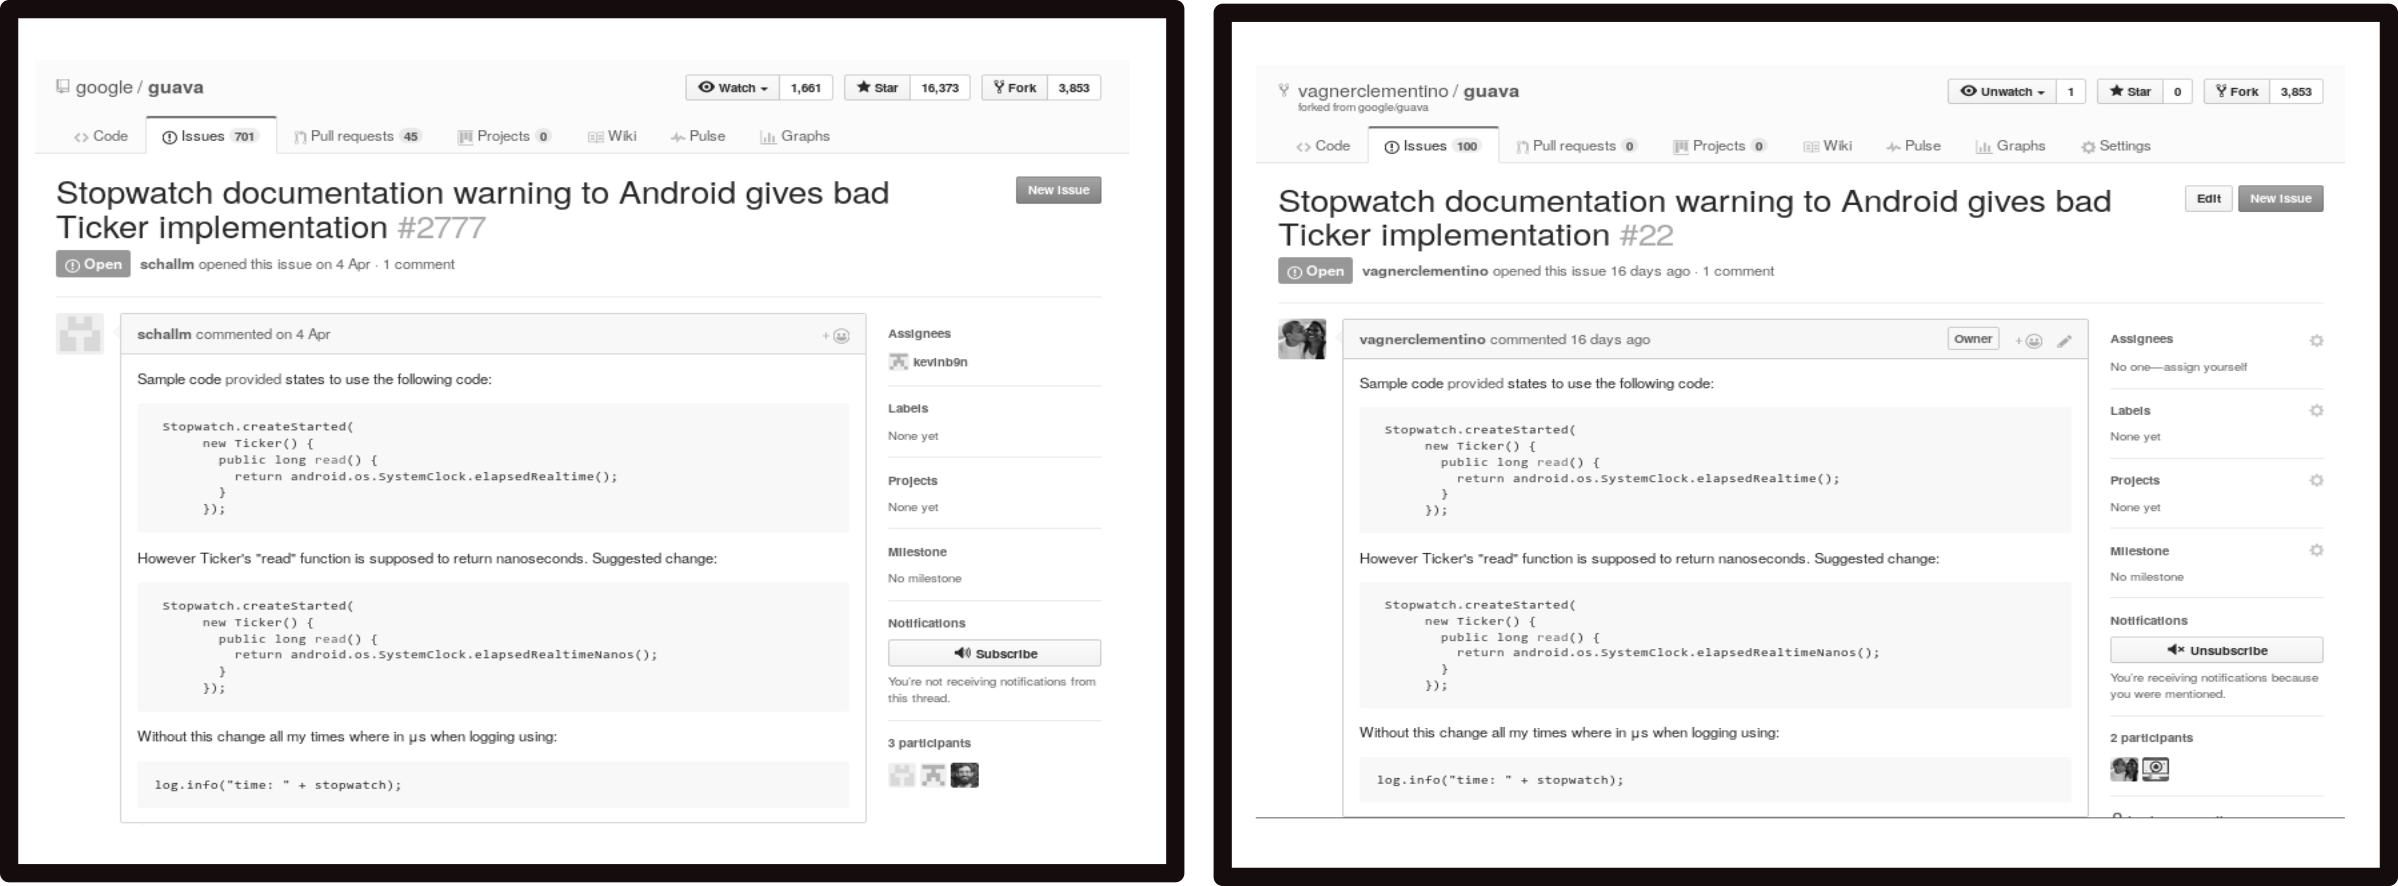
\includegraphics[width=1.1\linewidth]{chapter-implementacao-extensoes-fgrm/img/copia-de-issues.png}
    \caption{Cópia de uma RM do projeto Guava para a sua ramificação.}
\label{fig:copia-de-issues}
\end{figure}

Após finalizado o processo de cópia executamos a extensão com as 100
\textit{RMs} de cada projeto. Na Figura~\ref{fig:exemplo_comentario_issue}
visualizamos o comentário gerado para a \textit{RM} apresentada na
Figura~\ref{fig:copia-de-issues}. Na próxima seção apresentamos algumas métricas
do processo de execução da extensão nos projetos escolhidos. Como se trata de
uma prova de conceito estes dados podem nos ajudar na avaliação da viabilidade
de implantação da extensão proposta.

\begin{figure}[htpb]
    \centering
    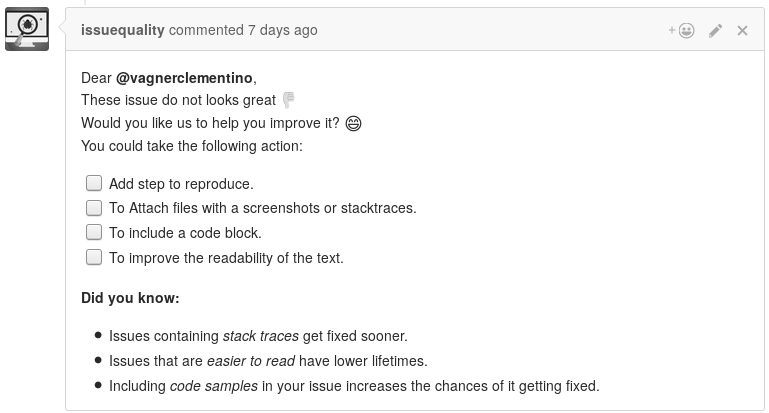
\includegraphics[width=0.7\linewidth]{chapter-implementacao-extensoes-fgrm/img/exemplo_comentario_issue.png}
    \caption{Comentário para a RM do projeto Guava exibida na Figura~\ref{fig:copia-de-issues}}
\label{fig:exemplo_comentario_issue}
\end{figure}

\subsection{Resultados}
\label{sub:implementacao_extensao_avaliacao_resultados}

Uma possível preocupação com a inclusão deste tipo de extensão em uma FGRM é a o
atraso que possa ocorrer no processo de solução das RMs. É natural que um tempo
adicional seja necessário para analisar a qualidade do relato. A
Tabela~\ref{tab:tempo_execucao_extensao} exibe o tempo em segundos que a
extensão levou para analisar as \textit{RMs}. É possível verificar que em
média cerca de 02 segundos são necessários para avaliar a qualidade do relato.
Em alguns casos o processo é finalizado em menos de 01 segundo. Entretanto, é
possível verificar situações em que o tempo de retorno da extensão é cerca de 30
segundos. Em alguns casos esta discrepância é maior, como no caso do projeto
\textit{Guava} que possui um desvio padrão acentuado em que o tempo de execução
pode variar de 01 a 31 segundos.

\begin{table}[htpb]
\centering
\resizebox{\textwidth}{!}{%
\begin{tabular}{@{}lccccc@{}}
\toprule
\multicolumn{1}{c}{\textbf{Projeto}} & \textbf{Média (seg.)} & \textbf{Mediana
    (seg.)} & \textbf{Desvio Padrão (seg.)} & \textbf{Min (seg.)} & \textbf{Max
    (seg.)} \\ \midrule
Todos & 1,91 & 1 & 2,93 & 0 & 31 \\
spring-framework & 2,36 & 1 & 4,13 & 1 & 31 \\
guava & 1,71 & 1 & 1,9 & 0 & 16 \\
elasticsearch & 1,66 & 1 & 2,24 & 0 & 16 \\ \bottomrule
\end{tabular}%
}
\caption{Tempo de execução da extensão.}
\label{tab:tempo_execucao_extensao}
\end{table}

Com a execução utilizando os dados de \textit{RMs} de projetos reais queríamos
de verificar em qual atributo do relato os problemas são mais frequentes.
Conforme apresentado na Tabela~\ref{tab:criterios_analise_qualidade_relato} a
extensão avalia os seguintes atributos do relato: Etapas para Reproduzir,
Arquivo Anexado, Fragmentos de Código, Completude de Palavras-Chaves e
Legibilidade do Texto. Um comentário é gerado caso o relato não atenda a
determinados critérios para cada atributo analisado. A
Figura~\ref{fig:frequencia_atributos_comentario} exibe a frequência que um item
foi incluído no comentário para atributo.

\begin{figure}[htpb]
    \centering
    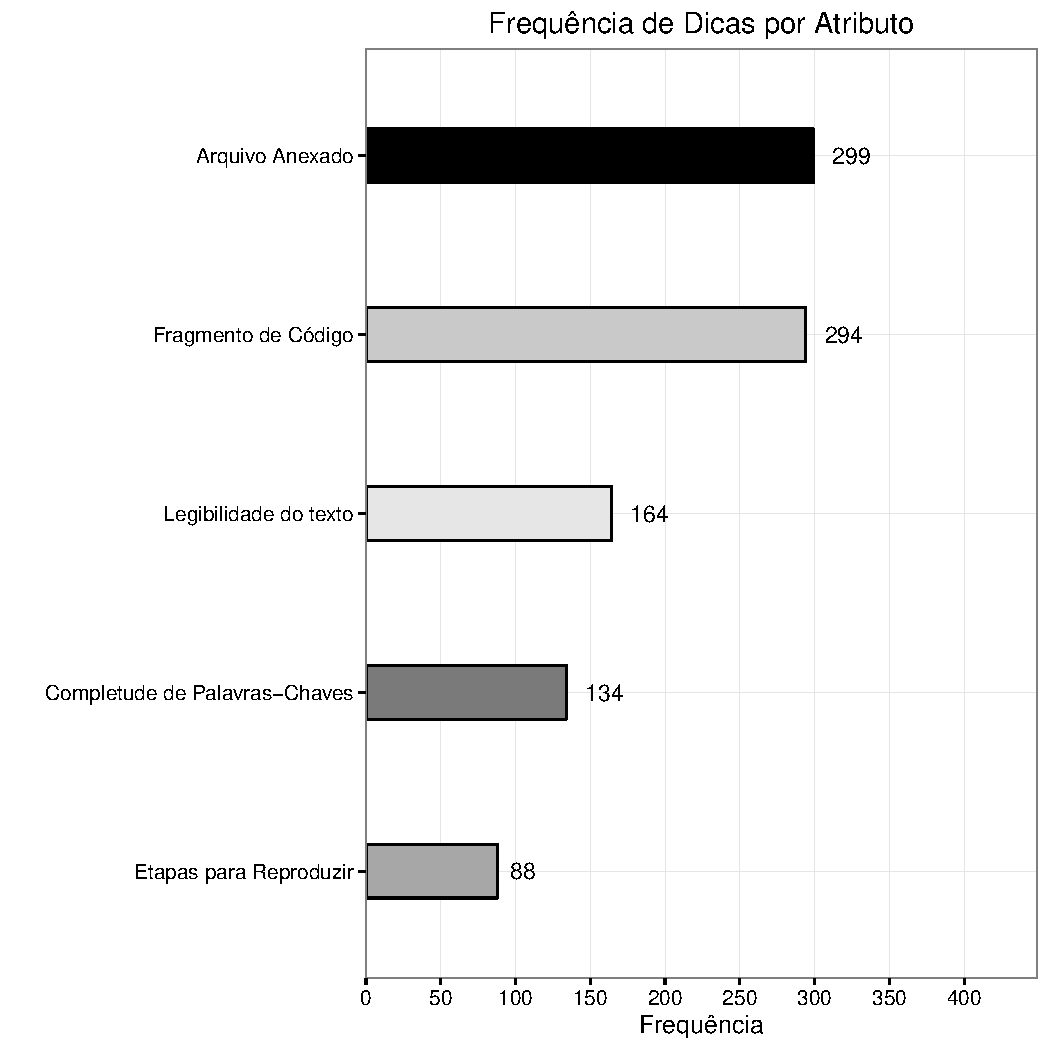
\includegraphics[width=0.5\linewidth]{chapter-implementacao-extensoes-fgrm/img/grafico_implementacao_extensao_freq_dicas_atributo.pdf}
    \caption{Frequência de dicas por atributo analisados.}
\label{fig:frequencia_atributos_comentario}
\end{figure}

Verificamos na figura que em quase todas as RMs analisadas não foi detectada a
inclusão de arquivos anexados ou de fragmentos de código. É possível observar
que mais da metade do texto relatado apresentou uma legibilidade ruim do ponto
de vista da nossa extensão. A situação menos frequente está relacionada com a
inclusão de ``Etapas para Reproduzir'', em que é avaliada a existência de uma
lista detalhando os passos executados até a ocorrência da falha.

\begin{table}[htpb]
\centering
\resizebox{\textwidth}{!}{%
\begin{tabular}{@{}lccccc@{}}
\toprule
\multicolumn{1}{c}{\textbf{Projeto}} & \textbf{Média (seg)} & \textbf{Mediana
    (seg)} & \textbf{Desvio Padrão (seg)} & \textbf{Min (seg)} & \textbf{Max
    (seg)} \\ \midrule
Todos & 3,26 & 3 & 0,96 & 1 & 5 \\
elasticsearch & 2,95 & 3 & 0,85 & 1 & 5 \\
guava & 3,16 & 3 & 0,88 & 2 & 5 \\
spring-framework & 3,68 & 4 & 1,01 & 1 & 5 \\ \bottomrule
\end{tabular}%
}
\caption{Número de dicas retornadas pela extensão.}
\label{tab:numero_de_dicas}
\end{table}

Durante a execução estávamos interessados em avaliar o número de dicas de
melhorias na qualidade do relato que a extensão gerou. Esta informação está
exibida na Tabela~\ref{tab:numero_de_dicas}. É possível observar que em média 03
dicas são incluídas em cada \textit{RM}, ou seja, três em cada cinco dos itens
apresentaram algum tipo de problema. Entretanto, para que possamos extrapolar
qualquer discussão sobre este resultado era necessário uma avaliação de pessoas
envolvidas nos projetos utilizados de modo a detectar falsos positivos.

\subsection{Discussão}
\label{sub:implemtacao_extensao_avaliacao_discussao}

As execuções que foram realizadas têm como foco avaliar a viabilidade da
extensão proposta. Neste sentido, os resultado obtidos na
Seção~\ref{sec:avaliando_a_extensao_proposta} devem ser avaliados sobre esta
ótica. No caso do tempo necessário verificamos que em média não causa impacto no
processo de solução de uma RM\@. Nos casos de maior duração, como por exemplo 31
segundos, pode estar relacionado a arquitetura escolhida. Conforme exposto, a
extensão utiliza uma API do Github está sujeita a questões relativas à rede ou
mesmo de sobrecarga.

Com relação aos problemas mais frequentes uma tendência dos usuário em não
incluir anexos, mas de relatar o problema copiando, por exemplo, as mensagens
contendo a cadeia de registros de ativação no próprio corpo da \textit{RM}. Por
outro lado, um fator a destacar é que mais da metade das \textit{RMs} analisadas
apresentam um texto com baixa legibilidade. Esta situação já foi verificada em
estudos anteriores~\cite{ko2006linguistic, bettenburg2007quality}. Esta métrica
depende menos de uma análise de alguém vinculado ao projeto pelo fato de
utilizar índices existentes e utilizados em diversas áreas para medir
legibilidade. Neste sentido pode ser interessante ao projeto de software
disciplinar os reportadores em fornecer sempre que possível um relato mais
simples e direto.

\section{Limitações e Ameças à Validade}
\label{sec:limitações_e_ameças_à_validade}

O desenvolvimento da extensão possui limitações que ameaçam a sua validade.
Inicialmente não é possível determinar se os atributos avaliados são os mais
indicados para medir a qualidade do relato. Eles foram utilizados com base em
estudos já realizados~\cite{bettenburg2007quality} em que os atributo foram
baseados na opinião de desenvolvedores.

Para que uma dica de melhoria seja disparada é necessário que um ou mais dos
critérios descritos na Tabela~\ref{tab:criterios_analise_qualidade_relato} não
sejam atendidos. No caso do atributo ``Completude de Palavras-Chaves''
utilizou-se o conjunto de termos do trabalho de Ko e
outros~\cite{ko2006linguistic}. Apesar de ambos os estudos utilizarem projetos
desenvolvidos na linguagem Java não podemos garantir que o conjunto de termos é
o mesmo nas RMs de diferentes projetos.

A legibilidade do texto foi implementada considerando testes descritos na
literatura. Em todos os testes existem os limiares que definem o grau de
legibilidade de um texto. Entretanto, não sabemos qual o impacto de utilizarmos
estes valores no relato de uma falha de software, por exemplo. Em geral, os
testes de legibilidade são bastante genéricos, contudo, certas adequações podem
ser necessárias para serem utilizados na análise do relato de uma RM\@.

A principal limitação deste estudo está na extrapolação dos resultados. O ideal
é que a execução da extensão fosse avaliada por um profissional vinculado aos
projetos utilizados. Esta análise poderia ajudar na detecção de falsos
positivos, por exemplo.

% Estendemos a importância deste tipo de suporte, mesmo que por inspeção de alguns
% casos. Um trabalho futuro desta dissertação seria reaplicar a extensão em uma
% configuração com suporte de um oráculo ligado ao projeto analisado.

\section{Conclusão}
\label{sec:implementacao_extensao_conclusao}

Neste capítulo discutimos alguns dos aspectos envolvidos na implementação de
melhorias de funcionalidades de FGRMs. Entendemos que existem vários aspectos
que não foram discutidos, como por exemplo planejamento de capacidade e
segurança, mas acreditamos que foram explicitados alguns aspectos importantes.

% \section{Resumo do Capítulo}
% \label{sec:implemtacao_extensao_resumo}
